\documentclass[11pt,fleqn]{article}

%% This first part is the document header, which you don't need to edit.
%% Scroll down to \begin{document} 

\usepackage[latin1]{inputenc}
\usepackage{enumerate}
\usepackage[hang,flushmargin]{footmisc}
\usepackage{amsmath}
\usepackage{amsfonts}
\usepackage{amssymb}
\usepackage{amsthm}
\usepackage{graphicx}
\graphicspath{{images/}}
\usepackage{url}

\theoremstyle{definition}
\newtheorem{theorem}{Theorem}
\newtheorem{lemma}[theorem]{Lemma}
\newtheorem{corollary}[theorem]{Corollary}
\newtheorem{proposition}[theorem]{Proposition}
\newtheorem{definition}[theorem]{Definition}
\newtheorem{example}[theorem]{Example}

\setlength{\oddsidemargin}{0px}
\setlength{\textwidth}{460px}
\setlength{\voffset}{-1.5cm}
\setlength{\textheight}{20cm}
\setlength{\parindent}{0px}
\setlength{\parskip}{10pt}

\begin{document}
\begin{center}
{\Huge
Setting Up the Git Environment
}\\
Aravind Koneru
\end{center}

\section*{Intro}

When we last met, I talked to you guys about some basic git functions and how to use them. This year
we will be working with git and github to create a sort of ``engineering notebook'' for our code and
it is important that all of you have the correct environment set up so that you are ready to
contribute to the code base. If some of this stuff seems overwhelming or you have no idea what's
happening, don't worry. Come talk to me and I can explain some of this stuff in more detail.
Throughout this setup guide, I'm going to assume that you have git installed and are semi
comfortable working in the command line (linux or osx). If you are using windows, the concept is
going to be the same but you will be running all these commands in the git terminal as opposed to
command prompt. 

\section*{Creating a fork}

\begin{enumerate}
\item
Create a github account if you don't already have one

\item
Go to this url:\\
\url{https://github.com/aravindkoneru/FTC_9042}\\
and you should see something like this

\begin{center}
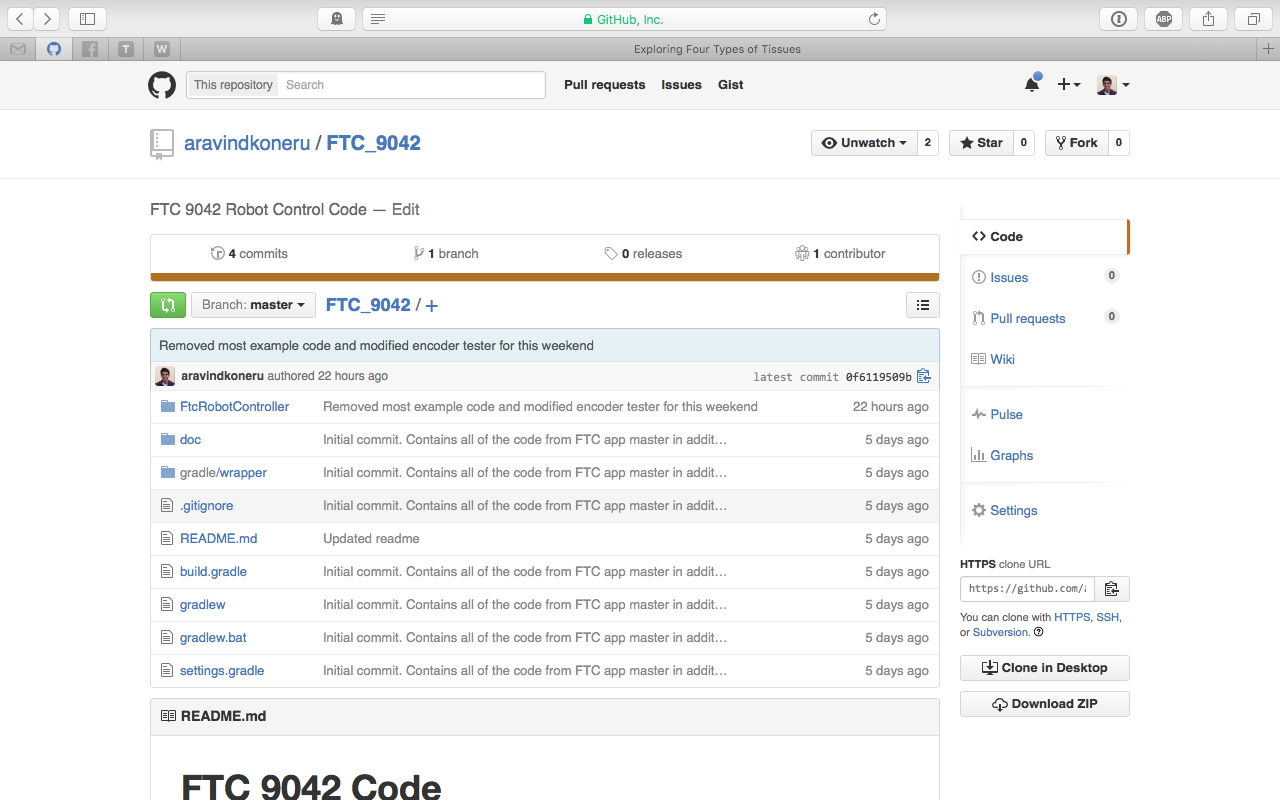
\includegraphics[scale=.35]{fork}
\end{center}

\item
Click the fork button in the top right hand corner

\item
Go back to your profile and you should now see that you have a repository named FTC9042 that is
forked from aravindkoneru/FTC9042
\end{enumerate}

Congratulations, you forked my repo!

\section*{Setting Up the Project}
\begin{enumerate}
\item
Open terminal (or git shell if on windows). Regardless of your OS, all the follow steps are the
same. 

\item
\texttt{cd} into the directory where you want to store the code. I personally work with a few
projects at a time so I like to have a git folder in my home directory that contains any projects
that I'm working on. On the bottom right you should see an option that says ``HTTPs clone url''. In
terminal type in \\
\texttt{git clone ...}\\
where ``...'' is the url you copied from github.  

\item
Now you should see that you a folder that contains all of the code from the repo. \texttt{cd} into
that folder and type 

\end{enumerate}

\end{document}
